\chapter{Autómatas con Transiciones Epsilon}
Extenderemos la definición de los AFND para incluir transiciones de un estado a otro que no dependen de ninguna entrada.

\textbf{Notación: }AFND-$\varepsilon$

\textbf{Definición: }Formalmente un AFND-$\varepsilon$ es una quíntupla $N=(S,I,\delta,s^*,F)$ donde $S,I,s^*,F$ se definen como en los AFND. $\delta$ es una función total de $(S\times I \cup\{\varepsilon\} \rightarrow P(s))$\\

\textbf{Ejemplo: }El siguiente AFND-$\varepsilon$ (Figura \ref{img_11_1}), $I=\{0,1,2\}$

%grafico1
\begin{figure}[h!]
\centering
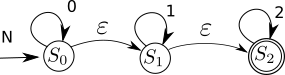
\includegraphics[width=0.5\textwidth]{img_11_1.png}
\caption{Diagrama de Transición} \label{img_11_1}
\end{figure}
$$L(N)=\{0^m1^n2^p/m\geq0,n\geq 0,p\geq 0\}$$

\textbf{Ejemplo: }Averiguar si la cadena $w=002$ es aceptada por el AFND-$\varepsilon$ $N$ (Figura \ref{img_11_1}), usando la definición recursiva.

\begin{align*}
\widehat{\delta}(s_0,\downlegend{0}{a}\downlegend{02}{u}) &=\widehat{\delta}(\delta(s_0,0),\downlegend{0}{a}\downlegend{2}{u})=\widehat{\delta}(s_0,02)=\widehat{\delta}(\delta(s_0,0),2) \\
&=\widehat{\delta}(s_0,\downlegend{2}{$\varepsilon 2$})=\widehat{\delta}(\delta(s_0,\varepsilon),2)=\widehat{\delta}(s_1,\downlegend{2}{$\varepsilon 2$})=\widehat{\delta}(\delta(s_1,\varepsilon),2)\\
&=\widehat{\delta}(s_2,2)=\delta(s_2,2)=s_2
\end{align*}

$w$ es aceptado por $N$, pues $s_2\in F$.

El camino que va de $s_0$ hacia $s_2$ es: 
$$s_0\rightarrow \downlegend{s_0}{0}\rightarrow \downlegend{s_0}{0}\rightarrow \downlegend{s_1}{$\varepsilon$}\rightarrow \downlegend{s_2}{$\varepsilon$} \rightarrow \downlegend{s_2}{2}$$

\textbf{Representación de un AFND}-$\varepsilon$: $\delta$ toma un estado de $S$ y un elemento de $I\cup \{\varepsilon\}$.

\textbf{Ejemplo: }Dibuje la tabla de transición para $N$
\begin{center}
$\begin{array}{c|cccc}
s		&0		&1		&2		& \varepsilon	\\ \hline
s_0		&s_0	&\phi	&\phi	&s_1	\\
s_1		&\phi	&s_1	&\phi	&s_2	\\
\sharp s_2	&\phi	&\phi	&s_2	&\phi
\end{array}$
\end{center}

\textbf{Definición: }Para todo estado $s\in S$ definimos la $\varepsilon$-clausura de $s$ como:
$$clausura_\epsilon(s)=\{ q/q \mbox{ es accesible desde }s\mbox{ sin consumir nada en la entrada} \}$$

\textbf{Nota: }El estado $s$ pertenece a $clausura_\epsilon(s)$.

\textbf{Ejemplo: }En el AFND-$\varepsilon$ $N$ (Figura \ref{img_11_1}) determine la clausura $\varepsilon$ para:

\begin{itemize}
\item $s=s_0$
\item $s=s_1$
\item $s=s_2$
\end{itemize}
\textbf{Solución: }
\begin{itemize}
\item $clausura_\varepsilon(s_0)=\{s_0,s_1,s_2\}$
\item $clausura_\varepsilon(s_1)=\{s_1,s_2\}$
\item $clausura_\varepsilon(s_2)=\{s_2\}$
\end{itemize}

Podemos extender la $\varepsilon$-clausura a un conjunto de estados $Q$ como sigue:
\begin{align*}
clausura_\varepsilon(Q)&=\bigcup_{q\in Q}clausura_\varepsilon(q)\\
clausura_\varepsilon(\{q_1,q_2,...,q_{i_N}\})&= \bigcup_{k=1}^N clausura_\varepsilon(q_{i_k})\\
Q\subseteq S
\end{align*}

\textbf{Ejemplo: }Dado el siguiente diagrama (Figura \ref{img_11_2}):

%grafico2
\begin{figure}[h!]
\centering
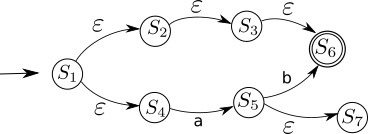
\includegraphics[width=0.5\textwidth]{img_11_2.png}
\caption{Diagrama de Transición} \label{img_11_2}
\end{figure}
Determine:
\begin{itemize}
\item $clausura_\varepsilon(s_1)$
\item El camino seguido para llegar a cada estado
\end{itemize}
\textbf{Solución: }
\begin{itemize}
\item $clausura_\varepsilon(s_1)=\{s_1,s_2,s_3,s_4,s_6\}$
\item
$\begin{array}{c|c}
s	&\mbox{camino}	\\ \hline
s_1	&s_1	\\
s_2	&s_1\rightarrow s_2	\\
s_3	&s_1\rightarrow s_2\rightarrow s_3	\\
s_4	&s_1\rightarrow s_4	\\
s_6	&s_1\rightarrow s_2\rightarrow s_3\rightarrow s_6
\end{array}$
\end{itemize}

\textbf{Definición: }La función de transición extendida a cadenas $\widehat{\delta}$ se define recursivamente:
\begin{itemize}
\item $\widehat{\delta}(s,\varepsilon)=clausura_\varepsilon(s)$
\item $\widehat{\delta}(s,ua)=clausura_\varepsilon(Q)$ Donde:

	$Q=\{q/\exists r\in \widehat{\delta}(s,u)\land q\in \delta(r,a)\}$
	
	$a\in I;u\in I^*;r,s\in S$ %%revisar
\end{itemize}

\textbf{Definición: }El lenguaje aceptado por un AFND-$\varepsilon$ $N=(S,I,\delta,s^*,F)$ es el conjunto.
$$L(N)=\{w/\widehat{\delta}(s^*,w)\land F\not= \phi\}$$

\textbf{Ejemplo: }Determine si $N$ acepta a la cadena $w=01$ en (Figura \ref{img_11_1}).

\textbf{Solución: }Hallamos primero $\widehat{\delta}(s_0,\varepsilon)$ y $\widehat{\delta}(s_0,0)$, $F=\{s_2\}$.
\begin{itemize}
\item $\widehat{\delta}(s_0,\varepsilon)=clausura_\varepsilon(s_0)=\{s_0,s_1,s_2\}$
\item \begin{align*}
\widehat{\delta}(s_0,\underbrace{0}_{\varepsilon 0})&=clausura_\varepsilon(\delta(\widehat{\delta}(s_0,\underbrace{\varepsilon}_{u}),\underbrace{0}_{a}))\\
&=clausura_\varepsilon(\delta(\{\underbrace{s_0,s_1,s_2}_{Q}\},0))\\
&=clausura_\varepsilon(\delta(s_0,0)\cup \delta(s_1,0)\cup \delta(s_2,0))\\
&=clausura_\varepsilon(s_0)=\{s_0,s_1,s_2\}
\end{align*}
Así:
\begin{align*}
\widehat{\delta}(s_0,\underbrace{0}_{u}\underbrace{1}_{a})&=clausura_\varepsilon(\delta(\widehat{\delta}(s_0,0),1))\\
&=clausura_\varepsilon(\delta(\{\underbrace{s_0,s_1,s_2}_{Q}\},1))\\
&=clausura_\varepsilon(\underbrace{\delta(s_0,1)}_{\phi}\cup \underbrace{\delta(s_1,1)}_{s_1}\cup \underbrace{\delta(s_2,1)}_{\phi})\\
&=clausura_\varepsilon(s_1)=\{s_1,s_2\}
\end{align*}
Como $\{s_1,s_2\}\cap F=\{s_2\}$, se acepta $w$.
\end{itemize}

\textbf{Definición: }Se define el conjunto de estado que siguen a $p$, pasando  por $\sigma$, mediante:
$$d(p,\sigma)=\{q/\mbox{hay una transición de }p\mbox{ a }q\mbox{ etiquetada por  }\sigma\}\qquad \sigma\in I$$

\textbf{Extensión}
$$d(\{\underbrace{p_{i_1},p_{i_2},...,p_{i_k},a}_{Q}\})=\bigcup_{j=1}^{k}d(p_{i_j},a)$$

\textbf{Ejemplo: }Sea el AFND-$\varepsilon$ dado el DT (Figura \ref{img_11_3}):

%grafico3
\begin{figure}[h!]
\centering
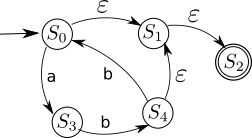
\includegraphics[width=0.4\textwidth]{img_11_3.png}
\caption{Diagrama de Transición} \label{img_11_3}
\end{figure}
$I=\{a,b\}$
$F=\{s_2\}$
Obtener:
\begin{itemize}
\item $\mbox{clausura}_\varepsilon(s_3) \qquad d(s_0,a)$
\item $\mbox{clausura}_\varepsilon(s_0) \qquad d(s_0,b)$
\item $\mbox{clausura}_\varepsilon(s_4) \qquad d(\{s_3,s_4\},b)$
\end{itemize}

\textbf{Solución: }
\begin{align*}
\mbox{clausura}_\varepsilon(s_3)	&=\{s_3\}	\\
\mbox{clausura}_\varepsilon(s_0)	&=\{s_0,s_1,s_2\}	\\
\mbox{clausura}_\varepsilon(s_4)	&=\{s_4,s_1,s_2\}	\\
d(s_0,a)	&=\{s_3\}	\\
d(s_0,b)	&=\phi	\\
d(\{s_3,s_4\},b)	&=d(s_3,b)\cup d(s_4,b)=\{s_4,s_0\}
\end{align*}